\subsection{Klassen-Diagramm}

    \begin{figure}[H]
        \centering
        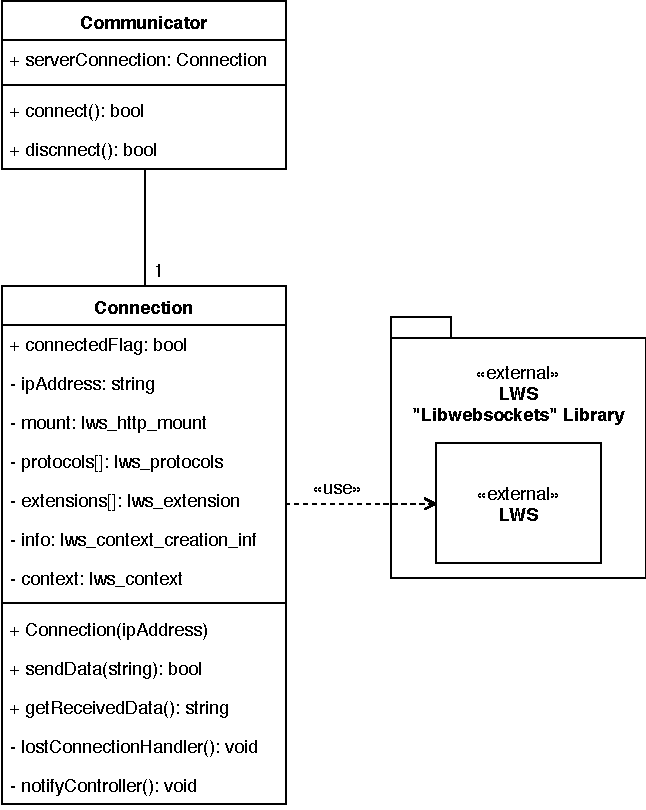
\includegraphics[scale=1]{images/Kommunikator.pdf}
    \end{figure}
    
    \newpage

\subsection{Beschreibung}
	\subsubsection{Connector (Klasse)}
	
		Im Allgemeinen dient die Connector Klasse dazu, die Kommunikation zwischen der Client Anwendung und der Server Anwendung über das Netzwerk zu verwalten. 
	
		\begin{description}
                
        	\item[connect (Methode)]
        	Die connect Methode dient dazu, eine neue Verbindung mit einem Server aufzubauen. Die IP-Adresse des Servers wird dabei als Parameter übergeben. Ist die Aktion erfolgreich, so wird true zurück gegeben, anderenfalls false.
			
			\item[disconnect (Methode)]
        	Die disconnect Methode dient dazu, eine bestehende Verbindung mit einem Server zu trennen. Ist die Aktion erfolgreich, so wird true zurück gegeben, anderenfalls false.
        	
    	\end{description}
	
	\subsubsection{Connection (Klasse)}    	
	
		\begin{description}
                
        	\item[sendData (Methode)]
        	Die öffentliche sendData Methode dient dazu, einen im JSON-Format formatierten String an den Server zu übertragen. Ist die Aktion erfolgreich, so wird true zurück gegeben, anderenfalls false. Zur Umsetzung dieser Methode werden Funktionen und Strukturen der Drittanbieter-Bibliothek LWS benötigt.
        	
        	\item[getReceivedData (Methode)]
			Mit Hilfe der öffentlichen Methode getReceivedData kann der letzte vom Server gesendete JSON Datensatz ausgelesen werden. Zur Umsetzung dieser Methode werden ebenfalls Funktionen und Strukturen der Drittanbieter-Bibliothek LWS benötigt.    	
        	
        	\item[lostConnectionHandler (Methode)]
			Die private Methode lostConnectionHandler kümmert sich im Falle eines außerplanmäßigen Verbindungsverlust darum, dass alle notwendigen Schritte eingeleitet werden, indem der Controller über den Verbindungsabbruch informiert wird. Auch hier werden zur Umsetzung Funktionen und Strukturen der Drittanbieter- Bibliothek LWS benötigt.          	
        	
        	\item[notifyController (Methode)]
        	Die private notifyController Methode ist dafür zuständig den Controller über das Eingehen von neuen Nachrichten des Servers zu informieren.
        	
    	\end{description}
    	
    \subsubsection{LWS (Externe Bibliothek)}
		Bei dieser Klasse Handelt es sich um eine externe Bibliothek, die verschiedenste Methoden und Strukturen zur Verfügung stellt um in einem C/C++ Projekt einfache Server Client Verbindungen mittels Web-Sockets zu implementieren. Genauere Informationen zu dieser Bibliothek sind unter folgendem Link zu finden: \\ \url{https://libwebsockets.org/}

\subsection{Zuordnung der Funktionalen Anforderungen}

Die Funktionalen Anforderungen werden den Methoden folgendermaßen zugeteilt:

\begin{table}[h]
	\centering
	\begin{tabular}{|l|l|}
    	\hline
    	\textbf{Funktionale Anforderungen} & \textbf{Methoden} \\ \hline
		FA55 & Connector::connect \\ \hline
    	FA55 & Connector::disconnect \\ \hline    	
    	FA55 & Connection::sendData \\ \hline
    	FA55 & Connection::getReceivedData \\ \hline
    	FA55 & Connection::lostConnectionHandler \\ \hline
    	FA55 & Connection::notifyController \\ \hline

	\end{tabular}
\end{table}